\begin{frame}{Introduction }
	\begin{columns}[c]
		\begin{column}{0.48\textwidth}
			
			\begin{itemize}
				\item Sleep stage classification is crucial for diagnosing sleep-related disorders.
				\item Processing raw EEG signals is computationally expensive and resource-intensive, especially with large datasets.
			\end{itemize}
		\end{column}
		\begin{column}{0.48\textwidth}
			\centering
			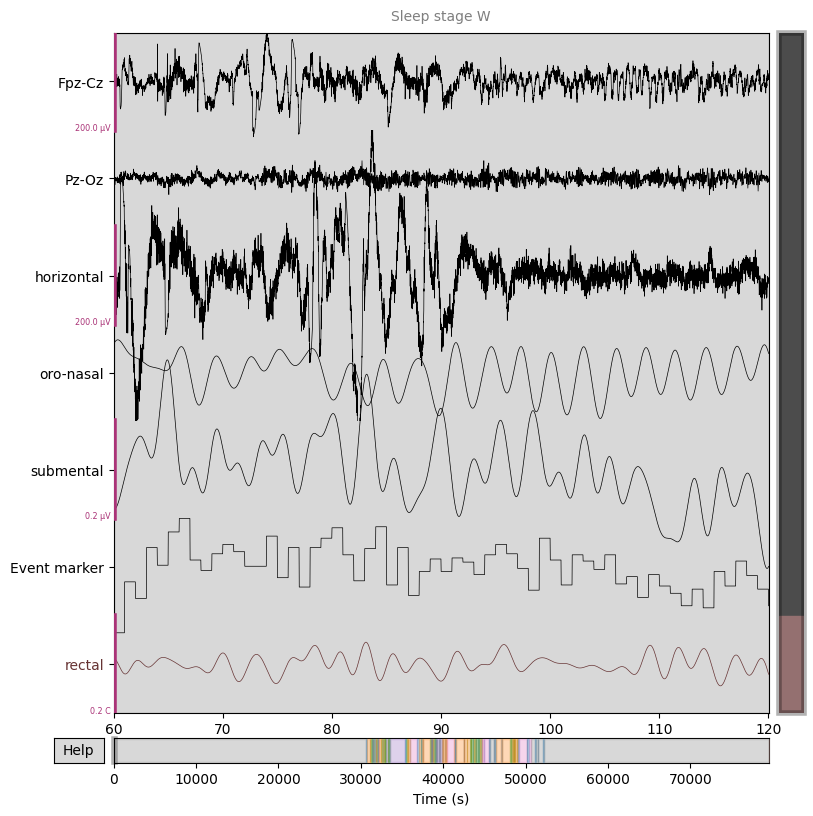
\includegraphics[width=0.9\textwidth]{images/paper_2/Sleep signals.png}
			\captionof{figure}{Visualization of EEG signal (PDEU)}
		\end{column}
	\end{columns}
\end{frame}

\begin{frame}{Introduction }
	\begin{columns}[c]
		\begin{column}{0.48\textwidth}
			
			\begin{itemize}
				\item This article discusses a method for preparing the Sleep-EDF dataset:
				\begin{itemize}
					\item Extracting, segmenting, and labeling PSG data.
					\item Converting data into Python pickle (\texttt{.pkl}) format for easy handling with deep learning frameworks.
				\end{itemize}
				\item Used annotation descriptions for sleep stage labeling.
			\end{itemize}
		\end{column}
		\begin{column}{0.48\textwidth}
			\centering
			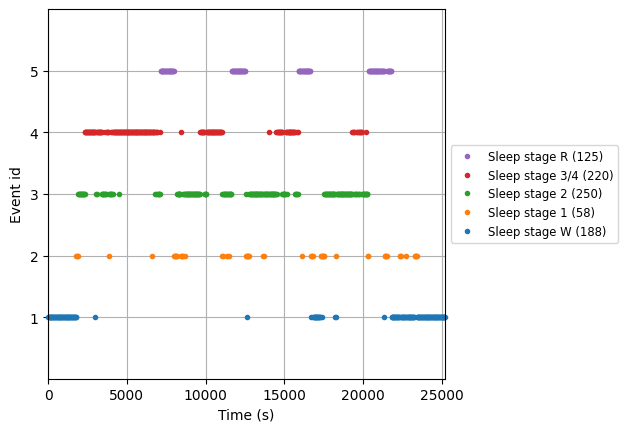
\includegraphics[width=0.9\textwidth]{images/paper_2/sleep event.png}
			\captionof{figure}{Sleep stage event plot}
		\end{column}
	\end{columns}
\end{frame}
